\pagebreak[5]
\subsection{The CML Metamodel (Abstract Syntax)}\label{subsec:metamodel}

The EMOF \cite{mof} model presented by figure \ref{fig:metamodel} is a simplified version of the CML metamodel:

\begin{figure}
\centering
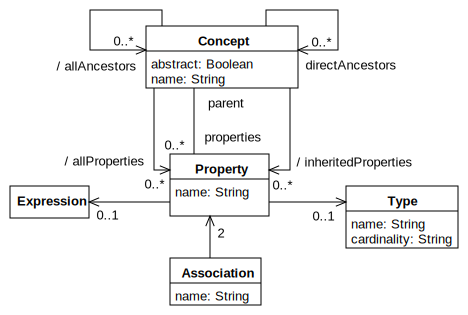
\includegraphics[width=0.8\textwidth]{language/diagram-metamodel}
\caption{This class diagram renders the EMOF \cite{mof} model defining the CML metamodel.}
\label{fig:metamodel}
\end{figure}


One key CML goal is to enabling the specification of conceptual models, such as those specified by ER \cite{er} models and UML \cite{url} class diagrams. In [article], [Author] shows how UML models, augmented by OCL constrains, can be used to specify conceptual models by mapping the UML/OCL metamodel to the ER metamodel. In order to present the CML concepts in the following subsections, a similar approach will be used by mapping the CML metamodel to the UML/OCL metamodels.

[Describe the relationships between the concepts in the diagram]

[Subsection for each key concept in the CML metamodel.]